% \section*{Введение}
% \addcontentsline{toc}{section}{\protect Введение}%
% IN PROGRESS...

% \RenewEnviron{equation}{
%   \settowidth{\myl}{$\BODY$}                       % calculate width and save as \myl
%   \origequation
%   \ifdimcomp{\the\linewidth}{>}{\the\myl}
%   {\ensuremath{\BODY}}                             % True
%   {\resizebox{\linewidth}{!}{\ensuremath{\BODY}}}  % False
%   \origendequation
% }


\section{Описание конструкции реактора}
ВВЭР-1000 конструктивно относится к классу гетерогенных корпусных реакторов. С точки зрения спектра нейтронов он является тепловым. В качестве теплоносителя и замедлителя используется легкая вода под давлением. В качестве топлива в реакторе используется низкообогащенным диоксид урана $UO_2$. Общий вид реактора в сборке представлен на рисунке \ref{pic:scheme}. 


В верхней части реактора расположена герметично закрытая крышка с установленными на ней приводами механизмов и органов регулирования и защиты. Также крышка оснащена патрубками для вывода кабелей датчиков внутриреакторного контроля. Крепление  к корпусу осуществляется с помощью шпилек. 


Реактор имеет двухконтурную систему. Энергия, выделяющаяся в результате ценой реакции деления ядер урана, преобразуется в тепловую энергию теплоносителя первого контура. Далее нагретый теплоноситель поступает с помощью тепловых насосов в парогенераторы, где происходит отдача тепла воде второго контура. Образовавшийся в парогенераторах пар далее поступает в паротурбинную установку, приводящую в движение турбогенератор, который вырабатывает электроэнергию.
% 
После передачи энергии в парогенераторах вода первого контура поступает в реактор через нижний ряд напорных патрубков. Сплошная кольцевая перегородка между рядами нижних и верхних патрубков, дистанцирующая корпус реактора и его шахту, формирует движение потока теплоносителя вниз. Поэтому вода проходит вниз по кольцевому зазору между корпусом и внутрикорпусной шахтой, затем через перфорированное эллиптическое днище и опорные трубы шахты входит в топливные тепловыделяющие сборки. Из ТВС через перфорированную нижнюю плиту блока защитных труб (БЗТ) теплоноситель выходит в межтрубное пространство БЗТ, а затем через кольцевой зазор между шахтой и корпусом и четыре верхних выходных патрубка из реактора.

%Параграф про водо-водянистость
%Параграф про корпусность
%Параграф про двухконтурность
%
\noindent
\begin{minipage}[t]{.5\textwidth}
\raggedright
\cite{лескин2011физические}
\begin{figure}[H]
	\begin{center}
		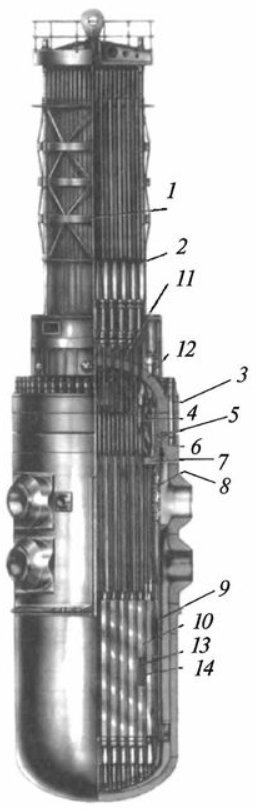
\includegraphics[scale=0.7]{Scheme.png}
		\caption{\small Общий вид реактора ВВЭР-1000 в сборе }
		\label{pic:scheme} % название для ссылок внутри кода
	\end{center}
\end{figure}
%
\end{minipage}%    <---------------- Note the use of "%"
\begin{minipage}[t]{.5\textwidth}
\raggedright
\begin{enumerate}
\item верхний блок; 
\item привод СУЗ;
\item шпилька;
\item труба для загрузки образцов-свидетелей;
\item уплотнение;
\item корпус реактора;
\item блок защитных труб;
\item шахта;
\item выгородка активной зоны;
\item топливные сборки;
\item теплоизоляция реактора; 
\item крышка реактора;
\item регулирующие стержни;
\item топливные стержни.
\end{enumerate}
\end{minipage}

\section{Теплофизический расчет}

\subsection{Постановка задачи}
В данном разделе будут определены основные термодинамические и гидравлические параметры реакторной установки. Теплофизический расчет подразумевает следующий ряд задач:

    \begin{enumerate}
        \item Выбор турбины и разработка принципиальной теплосиловой схемы установки;
        \item Рассчет КПД проектируемой установки;
        \item Рассчет основных теплофизических характеристик, таких как мощность ТВС и твэла, расход и скорость теплоносителя, коэффициент теплоотдачи;
        \item Построение распределения температур теплоносителя, оболочки и топлива по длинне для наиболее напряжённого канала; 
        \item Определение максимально возможных температур теплоносителя, оболочки и топлива;
        \item Рассчёт перепадов давлений и мощности, необходимой на прокачку теплоносителя;
        \item Рассчёт коэффициента запаса до кризиса теплообмена;
    \end{enumerate}

\subsection{Исходные данные для проведения расчетов}


Для проведения теплогидравлического расчета реакторной установки использовались следующие характеристики, представленные в Таблице \ref{tabular:data}.

\begin{table}[H]
	\caption{Исходные данные для проектируемого РУ ВВЭР-1000}
	\begin{center}
        \begin{tabular}{|l|c|}
        \toprule
         Характеристика & Значение \\ 
         \midrule
         \hline
         Электрическая мощность реактора, МВт & 1000 \\
         \hline\ 
         Температура теплоносителя на входе в АЗ $T_{\text{вх}}$, $^\circ C$  & 287 \\ 
         \hline\
         Температура теплоносителя на выходе АЗ $T_{\text{вых}}$, $^\circ C$ & 320 \\ 
         \hline
         Температура питательной воды, , $^\circ C$ & 220 \\ 
         \hline
         Температура свежего пара, $^\circ C$  &  274.6 \\ 
         \hline
         Давление свежего пара & 5.9 \\ 
         \hline
         Температура пара после пароперегревателей, $^○C$ & 250 \\ 
         \hline
         Давление в АЗ, МПа & 15.7 \\ 
         \hline
         Степень сухости пара после ЦВД и ЦНД, \% & 80 \\ 
         \hline
         Количество петель РУ & 4 \\ 
         \hline
         Число ТВС $N_{\text{ТВС}}$, шт  & 163 \\ 
         \hline
         Число твэл в ТВС $N_{\text{твэл}}$, шт & 317 \\ 
         \hline
         Коэффициент неравномерности по высоте АЗ  & 1.5 \\ 
         \hline
         Коэффициент неравномерности по радиусу АЗ & 1.25 \\ 
         \hline
         Высота АЗ $H_{\text{AZ}}$, м & 3.5 \\ 
         \hline
         Диаметр твэл $d_{\text{тв}}$, мм & 9.1 \\ 
         \hline
         Размер ТВС «под ключ» $a$, мм & 234 \\ 
         \hline
         Толщина чехла ТВС $\delta_{\text{чехла}}$, мм & 1.5 \\
         \hline
         Диаметр центрального канала в ТВС $D_{\text{ц.к}}$, мм & 10.3 \\ 
         \hline
         Число направляющих каналов в ТВС $N_{\text{н.к.}}$, шт & 12 \\ 
         \hline
         Шаг решетки ТВС $S_m$, мм & 12,75 \\ 
         \hline
         Диаметр направляющего канала в ТВС $D_{\text{н.к}}$, мм & 12.6 \\ 
         \hline
         Толщина оболочки твэл $\delta_{\text{твэл}}$, мм & 0.65 \\ 
         \hline
         Толщина газового зазора в твэл $\delta_{\text{г}}$, мм & 0.135 \\ 
         \hline
         Диаметр топливной таблетки $d_{\text{топ}}$, мм. & 7.53 \\ 
         \hline
         Диаметр отверстия топливной таблетки $d_{\text{\text{отв}}}$, мм & 1.3 \\ 
        %  \hline
        %  Число СУЗ $N_{\text{СУЗ}}$, шт & 109 \\ %сомнительная штука https://ru.wikipedia.org/wiki/%D0%92%D0%92%D0%AD%D0%A0-1000
        %  \hline
        %  Диаметр СУЗ $D_{\text{СУЗ}}$, мм & 8.2 \\
         \bottomrule
		\end{tabular}
		\label{tabular:data}
	\end{center}
\end{table}




\subsection{Выбор турбины}
В качестве турбины в расчетах будем использовать модель К-1000-60/1500-2. Её характеристики представлены в таблице \ref{tabular:turbine}

\cite{Андрушечко}
\begin{table}[H]
	\caption{Параметры турбины К-1000-60/1500-2 }
	\begin{center}
        \begin{tabular}{|l|c|}
        \toprule
         Параметр & Значение или Название \\ 
         \midrule
         \hline
         Прототип турбины &  К-1000-60/1500\\ 
         \hline
         Температура питательной воды, $^\circ C$ & 220 \\ 
         \hline
         Температура свежего пара, $^\circ C$  & 274.6\\
         \hline
         Давление свежего пара, $^\circ C$ & 5.9 \\ 
         \hline
         Температура после промежуточного перегрева, $^○C$ & 250 \\ 
         \hline
         Количество регенеративных подогревателей & 7 \\ 
         \bottomrule
		\end{tabular}
		\label{tabular:turbine}
	\end{center}
\end{table}


\begin{figure}[H]
	\begin{center}
		\includegraphics[scale=0.5]{teploscheme.jpg}
		\caption{Тепловая схема АЭС: 1 – ядерный реактор, 2 – главный
циркуляционный насос, 3 – парогенератор, 4 – цилиндр высокого давления, 5 –
сепаратор-пароперегреватель, 6 – цилиндры низкого давления, 7 – генератор, 8
– конденсатор, 9 – конденсационный электронасос, 10 – подогреватель низкого
давления, 11 – охладитель, 12 – станция насосная, 13 – деаэратор, 14 –
плунжерный электронасос, 15 – подогреватель высокого давления, 16 –
конденсационный насос с гидротурбинным приводом}
		\label{pic:teplocheme} % название для ссылок внутри кода
	\end{center}
\end{figure}


\subsection{Расчет КПД термодинамического цикла}


\begin{figure}[H]
	\begin{center}
		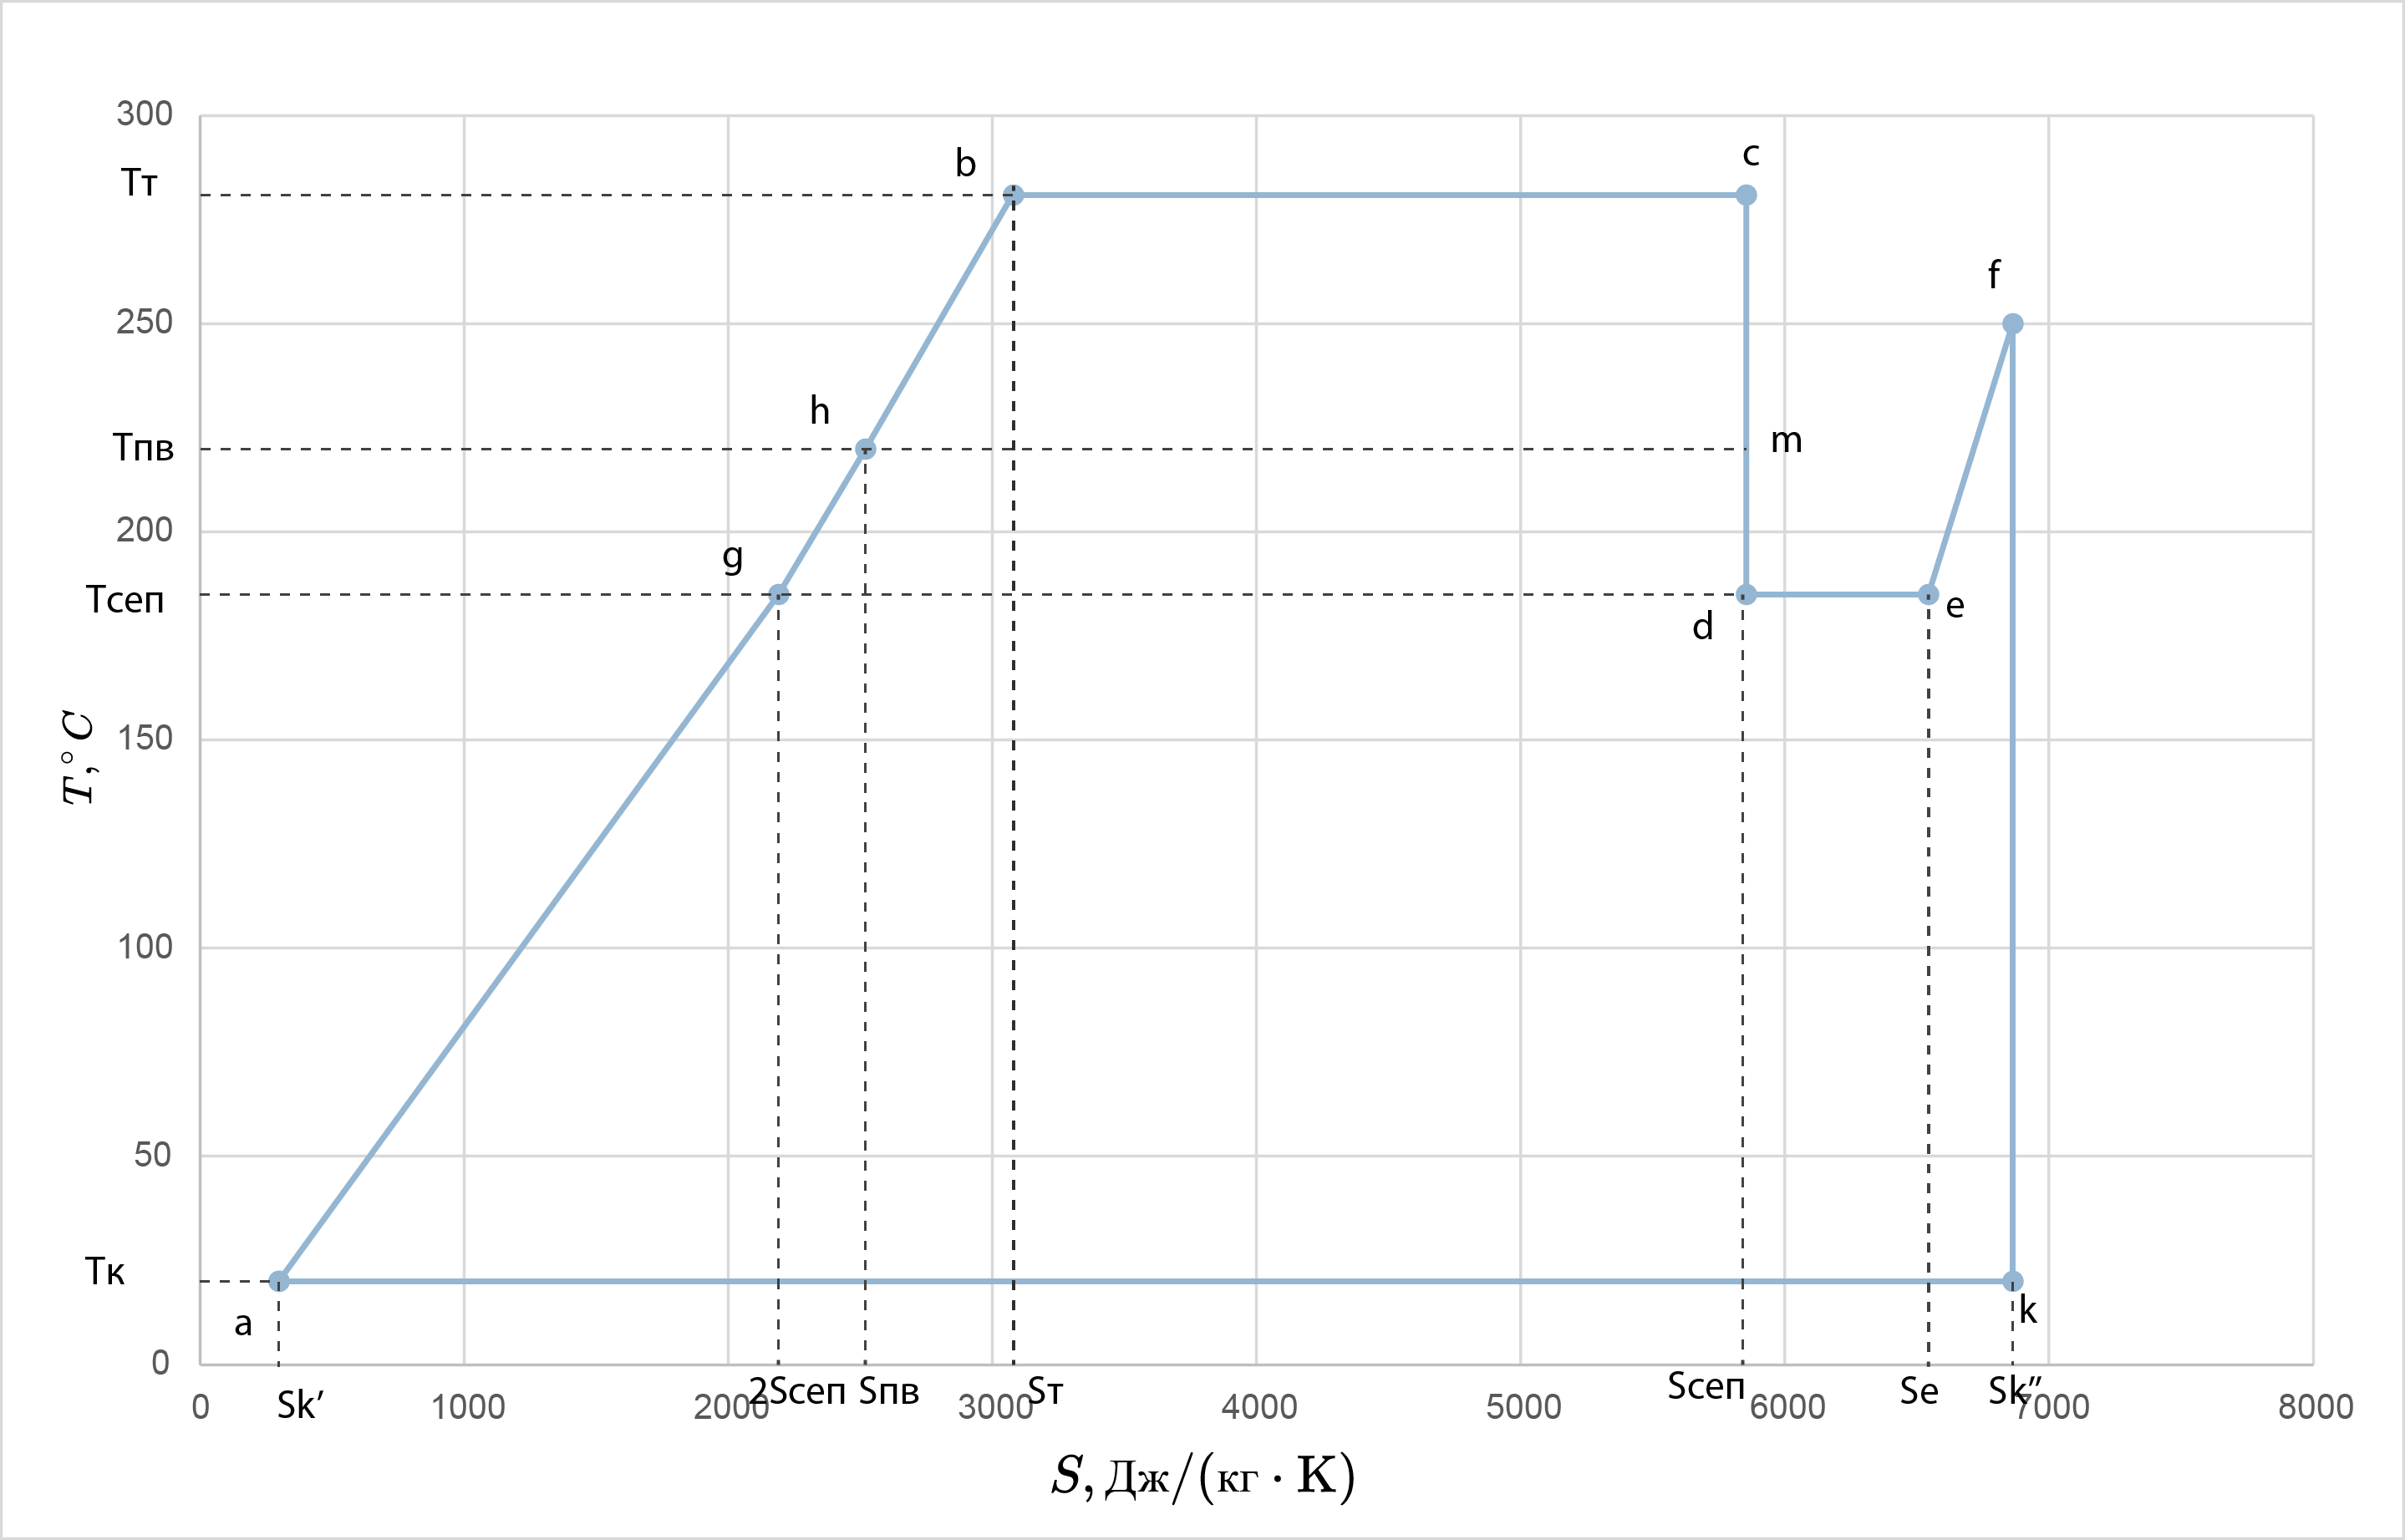
\includegraphics[scale=0.17]{TS.png}
		\caption{ T­S диаграмма турбинного цикла в реакторе ВВЭР­-1000 : hbc — нагрев и испарение в парогенераторе; cd — расширение пара в ЦВД; de — пар отделяется от конденсата в сепараторе; ef — пар поступает в промежуточный пароперегреватель; fk — расширение пара в ЦНД; ka — конденсация в конден­саторе; ag — регенеративный подогрев в ПНД; gh — регенеративный подогрев в ПВД;
        }
		\label{pic:TS} % название для ссылок внутри кода
	\end{center}
\end{figure}

\begin{table}[H]
	\caption{Значения параметров TS-диаграммы}
	\begin{center}
        \begin{tabular}{|c|c|c|c|c|}
        \toprule
         Точка & P, МПа & T, $^\circ C$ & S, Дж/(кг $\cdot$ К) & h, кДж/кг \\ 
         \midrule
         \hline
          h & 5.9 & 220 & 2516.4 & 942.9\\ 
         \hline
          b & 5.9 & 274.6 & 3017.4 & 1208.1 \\ 
         \hline
          c & 5.9 & 274.6 & 5898.01 & 2785.6\\ 
         \hline
          d & 0.98 & 179.189 & 5898.01 & 2462.7 \\ 
         \hline
          e & 0.98 & 179.189 & 6591.7 & 2776.4 \\ 
         \hline
          f & 0.98 & 250  & 6936.1 & 2943.61 \\ 
         \hline
          k & 0.004 & 28.7 & 6936.1 & 2099.5 \\ 
         \hline
          k′ & 0.004 & 28.7 & 416.66 & 119.656 \\ 
         \hline
          a & 5.9  & 28.7 & 414.9 & 125.1 \\ 
         \hline
          g & 0.98 & 179.2 & 2130.2 & 758.9 \\ 
         \bottomrule
		\end{tabular}
		\label{tabular:coeffs}
	\end{center}
\end{table}

Произведём расчет КПД для турбины К-1000-60/1500. Термический КПД без регенерации \cite{КирилловСправочник}:
\begin{equation}
\texteta_{t0}=1 - 
\frac{T_{k} ⋅ \left( s_{f} - s_{a} \right) ⋅ x_{d}}
{\left( h_{c} - h_{g} \right) +x_{d}\left( \left( h_{g} - h_{a} \right) + \left( h_{f} - h_{e} \right) \right)}
\end{equation}
\begin{equation}
\eta_{t0} = 
1 - 
\frac{3.017 \cdot 10^{ 2 } ⋅ \left( 6.936 \cdot 10^{ 3 } - 4.149 \cdot 10^{ 2 } \right) ⋅ 8.445 \cdot 10^{ -01 }}
{\left( 2.786 \cdot 10^{ 6 } - 7.589 \cdot 10^{ 5 } \right) + 8.445 \cdot 10^{ -01 } \left( \left( 7.589 \cdot 10^{ 5 } - 1.250 \cdot 10^{ 5 } \right) + \left( 2.944 \cdot 10^{ 6 } - 2.776 \cdot 10^{ 6 } \right) \right)}
\end{equation}
\begin{equation}
\eta_{t0}=3.854 \cdot 10^{ -01 }
\end{equation}

Термический КПД с идеальной регенерацией:

\begin{equation}
η_{t∞}=1 -
\frac{T_{k} ⋅ \left( s_{f} - s_{g} \right) \left( s_{c} - s_{h} \right)}
{\left(h_{c} - h_{h}\right) ⋅ \left( s_{e} - s_{g} \right) + \left( h_{f} - h_{e} \right) ⋅ \left( s_{c} - s_{h} \right)}
\end{equation}
\begin{equation}
η_{t∞}=
1 -
\frac{3.017 \cdot 10^{ 2 } ⋅ \left( 6.936 \cdot 10^{ 3 } - 2.130 \cdot 10^{ 3 } \right) \left( 5.898 \cdot 10^{ 3 } - 2.516 \cdot 10^{ 3 } \right)}
{\left(2.786 \cdot 10^{ 6 }) - 9.429 \cdot 10^{ 5 }\right) ⋅ \left( 6.592 \cdot 10^{ 3 } - 2.130 \cdot 10^{ 3 } \right) + \left( 2.944 \cdot 10^{ 6 } - 2.776 \cdot 10^{ 6 } \right) ⋅ \left( 5.898 \cdot 10^{ 3 } - 2.516 \cdot 10^{ 3 } \right)}
\end{equation}
\begin{equation}
η_{t∞}=4.420 \cdot 10^{ -01 }
\end{equation}

Термический КПД с $n = 7$  регенеративными отборами:
\begin{equation}
η_{tn} = η_{t0} + \left( η_{t∞} - η_{t0} \right) ⋅ \frac{n}{n+1}
=
3.854 \cdot 10^{ -01 } + \left( 4.420 \cdot 10^{ -01 } - 3.854 \cdot 10^{ -01 } \right) \cdot \frac{7}{8}
=4.349 \cdot 10^{ -01 }
\end{equation}

Учитываем:
$\eta^{\text{вн}}$ = 0.85 — внутренний КПД турбины;
$\eta_{\text{ос}}$ = 0.98 — коэффициент использования тепла, учитывающий; потери тепла в окружающую среду в прочем энергооборудовании;
$\eta_{\text{эг}}$ = 0.98 — КПД электрогенератора;
$\eta_{\text{мех}}$ = 0.97 — КПД механический,
Вычисляем КПД брутто АЭС как:
$$
\eta_{\text{брутто}} = \eta^7 \cdot \eta^{\text{вн}} \cdot \eta_{\text{ос}} \cdot \eta_{\text{эг}} \cdot \eta_{\text{мех}} = 0.335
=4.349 \cdot 10^{ -01 } \cdot 0.85 \cdot 0.98 \cdot 0.98 \cdot 0.97=3.444 \cdot 10^{ -01 }
$$
Тепловая мощность реактора при номинальной электрической мощности $Q_{\text{эл}} = 1000$ МВт равна:
$$
Q_{\text{теп}} = \frac{Q_{\text{эл}}}{\eta_{\text{брутто}}}=\frac{ 1.000 \cdot 10^{ 9 } } { 3.444 \cdot 10^{ -01 } } = 2.904 \cdot 10^{ 3 } \text{МВт}
$$


\subsection{Расчет изменения теплового потока в наиболее нагруженном канале}
из условия $$
K_z = \frac {\pi H_{\text{аз}}} {2 H_{\text{эф}} \sin \left(\frac {\pi H_{\text{аз}}}{2H_{\text{эф}}}\right)}  = 1.5
$$ 
находим эфективную добавку к высоте активной зоны. эффективная высота активной зоны будет равна $h_{\text{эф}} = 3.715$ м. максимальная величина теплового потока на один твэл:
\begin{equation}
q_{max} = \frac {Q_{\text{теп}}K_r K_z}{N_{\text{ТВС}}N_{\text{твэл}}H_{\text{аз}}}  
=
\frac 
{ 2.904 \cdot 10^{ 9 } \cdot 1.25 \cdot 1.5  }
{ 163 \cdot 317 \cdot 3.5 }
=3.010 \cdot 10^{ 2 } \frac {\text{Вт}} {\text{см}}
\end{equation}
Зависимость величины теплового потока от высоты:
$$
q(z) = q_{max}\cos\left(\frac {\pi\cdot z} {H_{\text{эф}}}\right) = 3.010 \cdot 10^{ 2 }\cos \left(\frac {\pi \cdot z} {3.715} \right)\ \left[\frac{\text{Вт}}{\text{см}} \right]
$$

\subsection{Расчет распределения температуры теплоносителя по высоте}

Энтальпия входа $h_{\text{вх}} =1.268 \cdot 10^6 \frac{Дж}{кг}$.%из wsp через F(P,T) температуру на входе и давление в АЗ.

\noindent Энтальпия выхода $h_{\text{вых}} =1.452 \cdot 10^6 \frac{Дж}{кг}$. %аналогично 

\noindent Расход теплоносителя через ТВС:
$$
G_{\text{ТВС}} = \frac {Q_{\text{теп}}} {(h_{\text{вых}} - h_{\text{вх}})N_{\text{ТВС}}}
=
\frac { 2.904 \cdot 10^{ 9 } } { ( 1.452 \cdot 10^{ 6 } - 1.268 \cdot 10^{ 6 }) \cdot 163 } = 9.685 \cdot 10^{ 1 } \ \frac {\text{кг}}{\text{c}}
$$
Расход теплоносителя через реактор:
$$
G_{\text{реак}} = \frac {Q_{\text{теп}}} {(h_{\text{вых}} - h_{\text{вх}})}
=
\frac { 2.904 \cdot 10^{ 9 } } { ( 1.452 \cdot 10^{ 6 } - 1.268 \cdot 10^{ 6 }) } = 1.579 \cdot 10^{ 4 } \ \frac {\text{кг}}{\text{c}}
$$
Средняя теплоемкость воды:
$$
C_p = \frac {h_{\text{вых}} - h_{\text{вх}}} {T_{\text{вых}} - T_{\text{вх}}}
=
C_p = \frac { 1.452 \cdot 10^{ 6 } - 1.268 \cdot 10^{ 6 } } { 5.930 \cdot 10^{ 2 } - 5.600 \cdot 10^{ 2 } } = 5.574 \cdot 10^{ 3 } \ \frac{ \text{Дж}} { \text{кг} \cdot \text{К} }
$$
\noindent Распределение температуры теплоносителя по высоте реактора:
$$
T_{ТН}(z) = T_{\text{вх}} + \frac {N_{\text{ТВС}}N_{\text{ТВЭЛ}}q_{\max}H_{\text{эф}}} {G_{\text{реак}}C_p\pi}\left[\sin \left(\frac {\pi z}{H_{\text{эф}}} \right) +\sin \left(\frac {\pi H_{\text{АЗ}}} {2H_{\text{эф}}} \right) \right]
$$
\noindent Отсюда максимальная температура жидкости $T_{\text{ТН}}^{max} = 328.54\  ^\circ C$.
График изменения температуры теплоносителя по высоте представлен на \ref{pic:TZ}

\begin{figure}[H]
	\begin{center}
		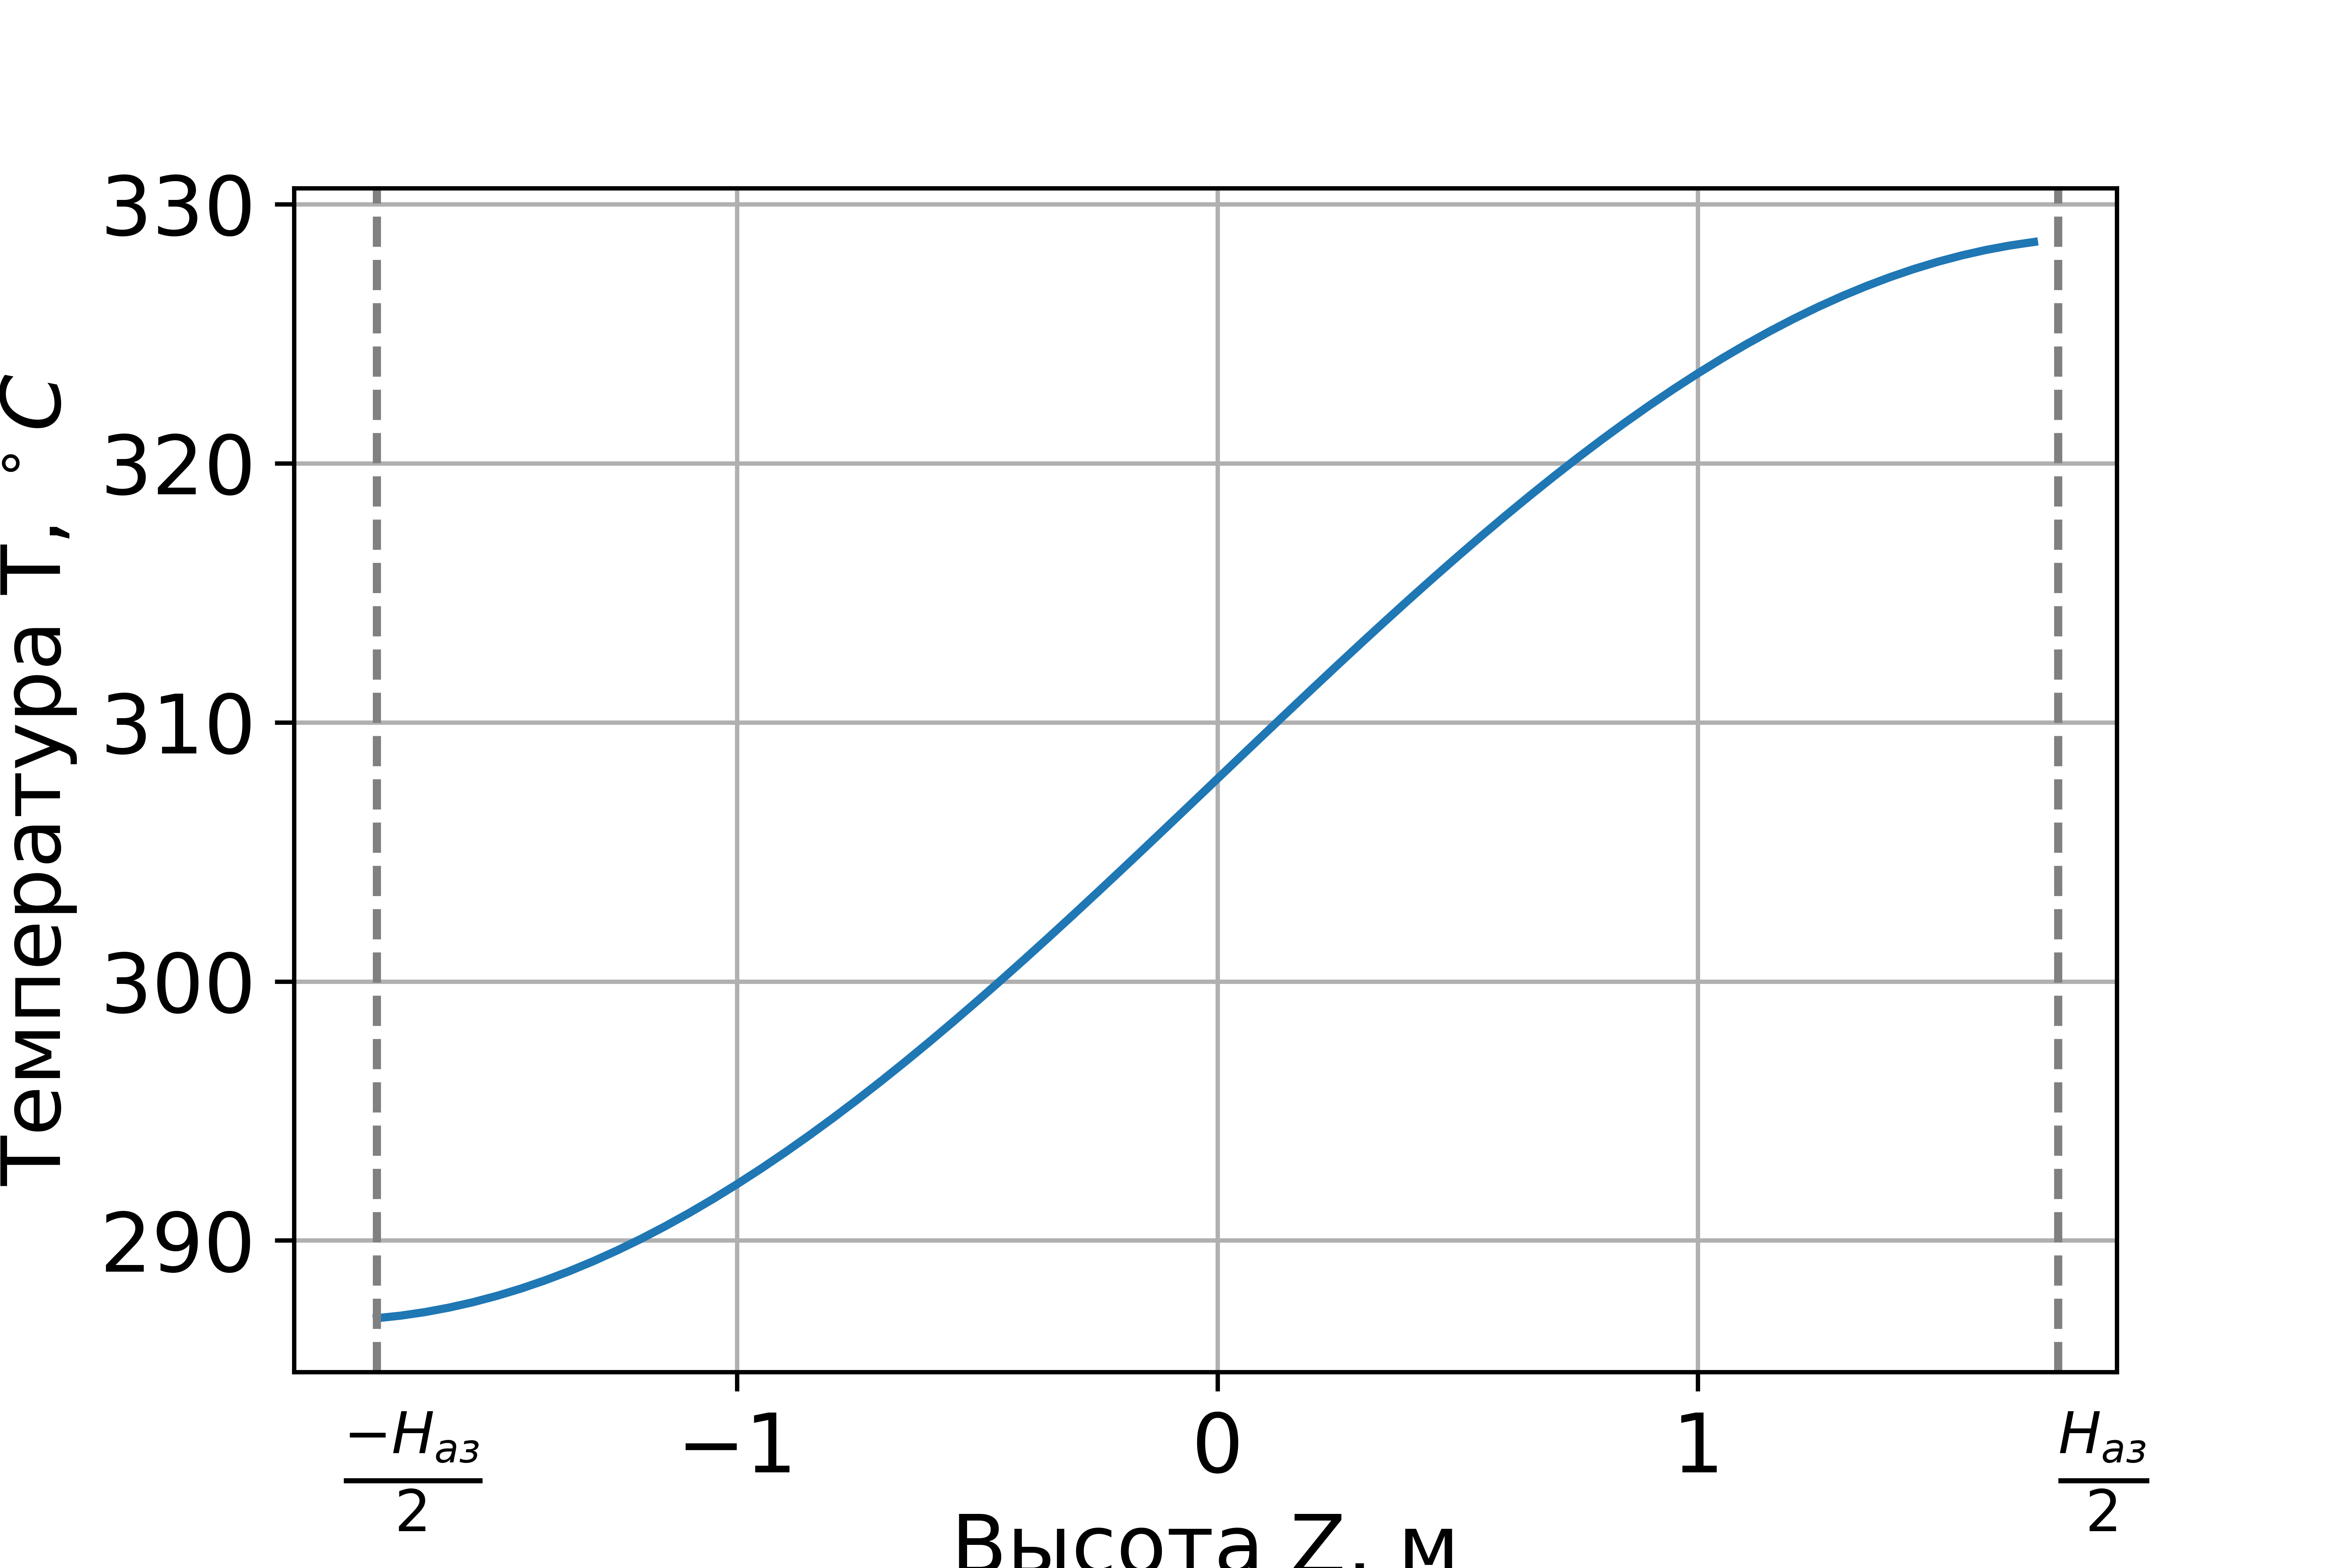
\includegraphics[]{Tz.png}
		\caption{Изменение температуры теплоносителя по высоте}
		\label{pic:TZ} % название для ссылок внутри кода
	\end{center}
\end{figure}

Максимальная температура теплоносителя определяется из температуры кипения теплоносителя при давлении в активной зоне. Температура насыщения воды при давлении $15.7$ МПа — $345.8\  ^\circ C$. Отсюда следует что запас до кипения $\approx 17.26\  ^\circ C$. 

\subsection{Расчет распределения температуры внешней стенки оболочки по высоте}
Площадь проходного сечения:
\begin{equation}
S_{\text{прох}} = \sqrt{3}/2(a - 2 \cdot \delta_{\text{чехла}})^2 - N_{\text{твэл}} \frac {\pi d^2_{\text{тв}}} {4} - N_{\text{н.к.}} \frac {\pi D_{\text{н.к}}^2} {4} - \frac {D_{\text{ц.к}}^2\pi}{4}
\end{equation}
\begin{equation}
S_{\text{прох}} =\sqrt{3}/2(2.340 \cdot 10^{ -01 } - 2 \cdot 0.0015)^2 - 3.170 \cdot 10^{ 2 } \frac { \pi (9.100 \cdot 10^{ -03 })^2 } {4} - 1.200 \cdot 10^{ 1 } \frac { \pi (1.260 \cdot 10^{ -02 }))^2} {4} - \frac { (1.030 \cdot 10^{ -02 })^2\pi } {4} 
\end{equation}
\begin{equation}
S_{\text{прох}} =  2.402 \cdot 10^{ 4 } \text{мм}^2
\end{equation}

Периметр:
\begin{equation}
\Pi= (2(a-2\delta_{\text{чехла}})\sqrt{3}) - N_{\text {твэл }} \pi d_{\text {тв }}+N_{\text {н.к }} \pi D_{\text {н.к }}+\pi D_{\text {ц.к}}
\end{equation}
\begin{equation}
\Pi=(2( \cdot 2.340 \cdot 10^{ -01 }-2 \cdot 1.500 \cdot 10^{ -03 }) \cdot \sqrt{3}) - 3.170 \cdot 10^{ 2 } \cdot \pi \cdot 9.100 \cdot 10^{ -03 } + 1.200 \cdot 10^{ 1 } \cdot \pi \cdot 1.260 \cdot 10^{ -02 } + \pi \cdot 1.030 \cdot 10^{ -02 }
\end{equation}
\begin{equation}
\Pi= 1.037 \cdot 10^{ 4 } \text{мм}
\end{equation}
Гидравлический диаметр:
$$
d_{\text{Г}} = \frac {4 S_{\text{прох}}}{\text{П}}
=
\frac {4 \cdot 2.402 \cdot 10^{ -02 }} {1.037 \cdot 10^{ 1 }} = 9.263 \cdot 10^{ -03 }
 \text{мм}
$$

Определим коэффициент теплоотдачи в режиме турбулентного
стационарного течения несжимаемой жидкости. 
Параметры теплоносителя при усредненной температуре $\overline{T}=303.5 ^\circ \mathrm{C}$:
\begin{itemize}
\item Динамическая вязкость $\mu = 8.721 \cdot 10^{-5} \text{Па} \cdot \text{c}$ 
\item Коэффициент теплопроводности $\lambda = 0.5536 \frac {\text{Вт}}{\text{м} \cdot K}$
\item Число Прандтля $Pr = 0.8729$
\end{itemize}

По формуле Б.С.Петухова, В.В. Кириллова (круглые трубы) \cite{богословская}:

Число Рейнолдса:
$$
\operatorname{Re}=\frac{G_{\text {реак }} \cdot d_{\mathrm{r}}}{N_{\mathrm{TBC}} \cdot S_{\text {npox }} \cdot \mu} = 4.283 \cdot 10^{ 5 }
$$
Коэффициент гидравлического сопротивления:
$$
\xi_{\text{тр}}=(1,82 \cdot \log (\mathrm{Re})-1.64)^{-2}= 1.35 \cdot 10^{-02}
$$
Расчитываем число Нуссельта:
\begin{align*}
\mathrm{Nu}=&\frac{\frac{\xi}{8} \cdot \mathrm{Re} \cdot \operatorname{Pr}}{k+12.7 \cdot\left(\operatorname{Pr}^{\frac{2}{3}}-1\right) \cdot \sqrt{\frac{\xi}{8}}}
=\\=&
\frac{ 
    \frac{1.349 \cdot 10^{ -02 }}{8} \cdot 4.283 \cdot 10^{ 5 } \cdot 8.729 \cdot 10^{ -01 } 
}
{ 
    1 + \frac{900}{4.283 \cdot 10^{ 5 }} + 12.7 \cdot\left((8.729 \cdot 10^{ -01 })^{\frac{2}{3}}-1\right) \cdot \sqrt{\frac{1.349 \cdot 10^{ -02 }}{8}} 
} = 6.589 \cdot 10^{ 2 }
\end{align*}, где $k = 1 + \frac{900}{Re}$  \\
Коэффициент теплоотдачи:
    $$
    \alpha_1 = \frac {Nu \cdot \lambda} {d_\text{г}} = \frac {6.589 \cdot 10^{ 2 } \cdot 5.536 \cdot 10^{ -01 }}{9.263 \cdot 10^{ -03 }} = 3.938 \cdot 10^{ 4 } \frac {\text{Вт}}{\text{м}^2\cdot\mathrm{K}}
    $$
По формуле Диттуса-Болтера \cite{деев}:
    $$
    Nu = 0.023Re^{0.8}Pr^{0.4} = 697.5
    $$
Коэффициент теплоотдачи:
    $$
    \alpha_2 = \frac {Nu \cdot \lambda} {d_\text{г}} = \frac {6.975 \cdot 10^{ 2 } \cdot 5.536 \cdot 10^{ -01 }}{9.263 \cdot 10^{ -03 }} = 4.169 \cdot 10^{ 4 } \frac {\text{Вт}}{\text{м}^2\cdot\mathrm{K}}
    $$
По формула М.А. Михеева \cite{михеев}:
    $$
    Nu = 0.021Re^{0.8}Pr^{0.43} = 634.28
    $$
Коэффициент теплоотдачи:
    $$
    \alpha_3 = \frac {Nu \cdot \lambda} {d_\text{г}} = \frac {6.343 \cdot 10^{ 2 } \cdot 5.536 \cdot 10^{ -01 }}{9.263 \cdot 10^{ -03 }} = 3.791 \cdot 10^{ 4 } \frac {\text{Вт}}{\text{м}^2\cdot\mathrm{K}}
    $$
Усредним коэффициент теплоотдачи:
    $$
    \alpha = \frac {\alpha_1 + \alpha_2 + \alpha_3} {3} = 3.966 \cdot 10^{ 4 } \frac{\text{Вт}}{\text{м}^2 \cdot K}
    $$
Распределение температуры внешней стенки твэла по высоте реактора:
    $$
    T_{\text {об }}(z)=T_{\text {тн }}(z)+\frac{q_{\max } \cdot \cos \left(\frac{\pi \cdot z}{H_{\ni \phi}}\right)}{\pi d_{\text {тв }} \alpha}
    $$
Распределение температуры внешней стенки
твэла по высоте реактора представлено на \ref{pic:Tob}

\begin{figure}[H]
	\begin{center}
		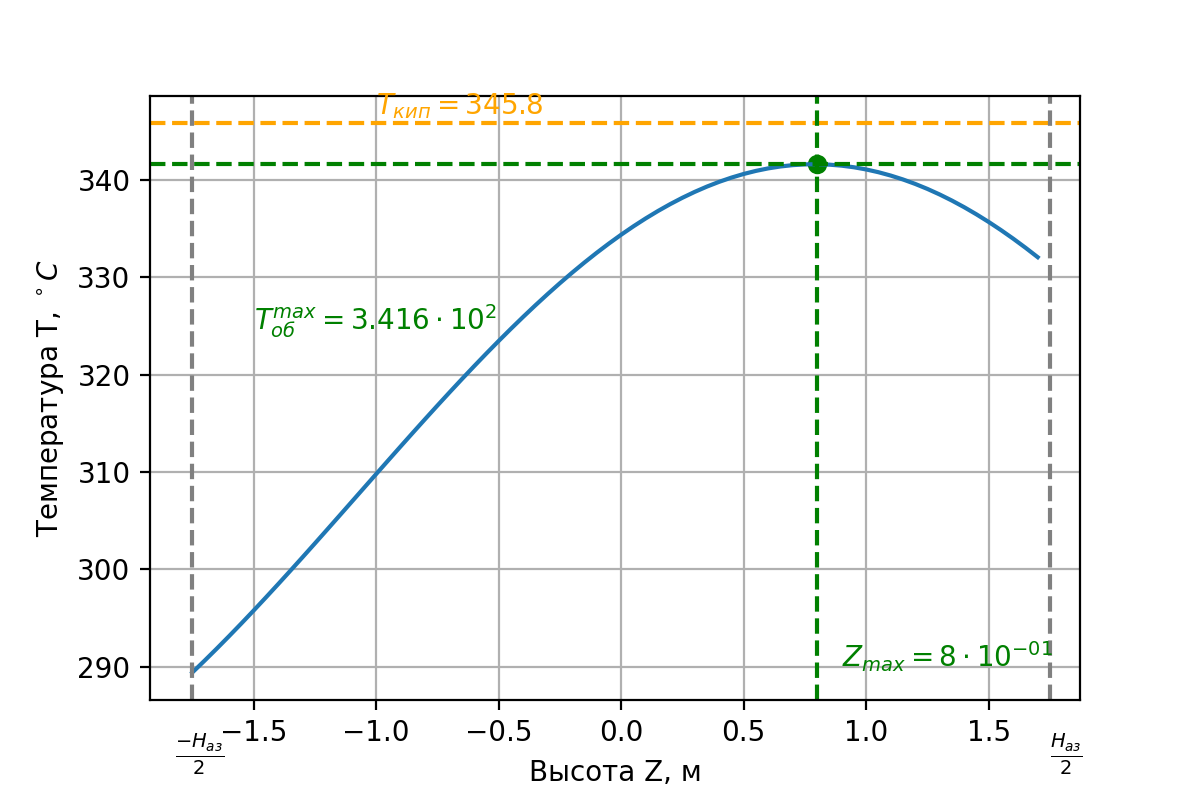
\includegraphics[]{Tob.png}
		\caption{Изменение температуры стенки твэла по высоте}
		\label{pic:Tob} % название для ссылок внутри кода
	\end{center}
\end{figure}

 Из \ref{pic:Tob} 
 видно, что максимальная температура $T_{\text{об}}^{\max} = 341.6 ^\circ C $ стенки достигается в $Z_{\max} = 0.8 м$. Отсюда можно сделать вывод о том, что также отсутствует поверхностное кипения теплоносителя.
 %максимальная температура оболочки в условиях нормальной эксплуатации определяется прочностными и пластическими свойствами сплава и составляет сколь-кот то из справочника

Общий график для распределений теплоносителя и оболочки представлены на \ref{pic:obsh}
\begin{figure}[H]
	\begin{center}
		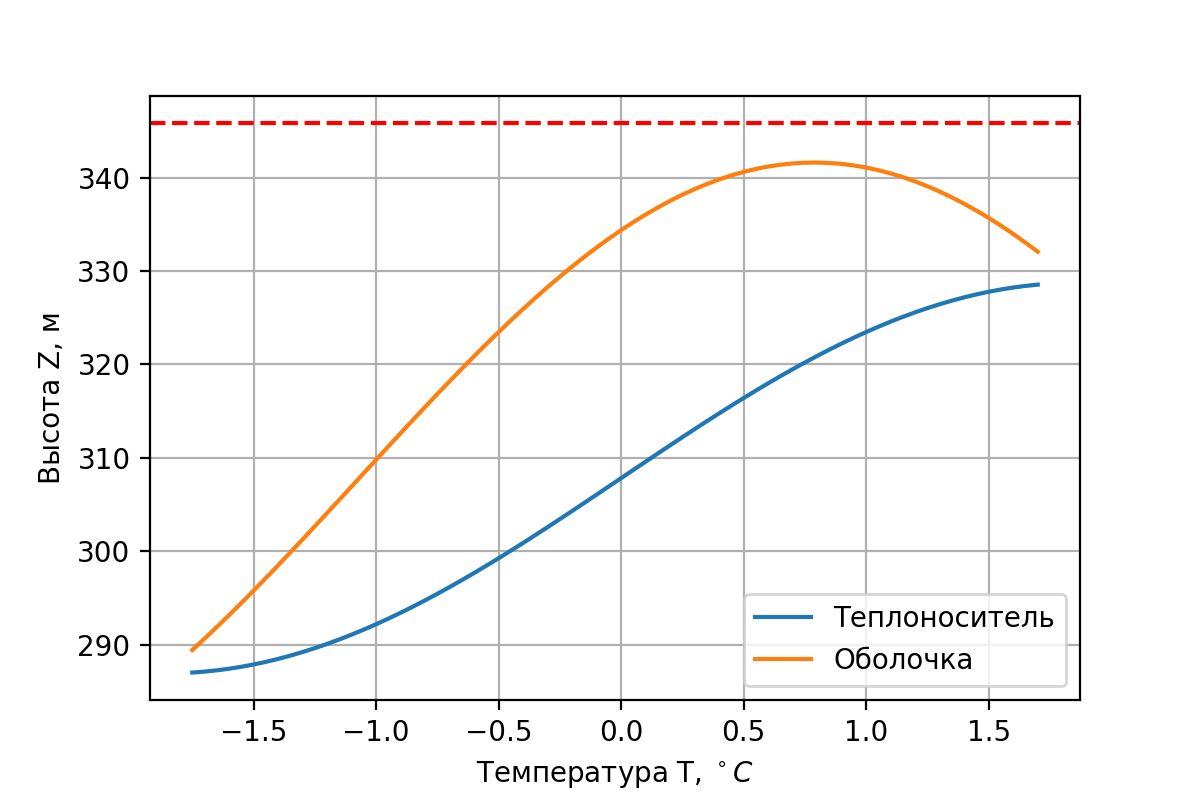
\includegraphics[]{Obsh.png}
		\caption{Изменение температуры стенки твэла и теплоносителя по высоте}
		\label{pic:obsh} % название для ссылок внутри кода
	\end{center}
\end{figure}
    
%NСУЗ — по числу отверстий в канале 

\subsection{Расчет температуры топлива}
    Произведём расчет термического сопротивления оболочки, газового зазора и топлива:
\begin{align*}
\sum R_i =& 
\frac {\ln \frac {d_{\text{тв}}}{d_{\text{тв}} - 2\delta_{об}}  }{2\pi\lambda_{\text{об}}}+\frac {\ln \frac {d_{\text{тв}} - 2\delta_{об}}{d_{\text{топ}}}  }{2\pi\lambda_{\text{г.з}}}+\frac {\frac 1 2 - \frac {d_{\text{отв}}^2} {d_{\text{топ}}^2 - d_{\text{отв}}^2}\ln \frac {d_{\text{топ}}}{d_{\text{отв}}}} {2 \pi \lambda_{\text{топ}}} =
=\\=&
\frac {\ln \frac{ 9.100 \cdot 10^{ -03 } }{ 9.100 \cdot 10^{ -03 } - 2 \cdot 6.500 \cdot 10^{ -04 }} } {2\cdot \pi \cdot 2.010 \cdot 10^{ 1 }}
\\+& \frac {\ln \frac {9.100 \cdot 10^{ -03 } - 2 \cdot 6.500 \cdot 10^{ -04 }}{7.530 \cdot 10^{ -03 }} } {2 \pi \cdot 3.500 \cdot 10^{ -01 }}
\\+& \frac { 0.5 - \frac{ (1.300 \cdot 10^{ -03 })^2 }{ (7.530 \cdot 10^{ -03 })^2 - (1.300 \cdot 10^{ -03 })^2 } \ln \frac { 7.530 \cdot 10^{ -03 } }{ 1.300 \cdot 10^{ -03 } } } {2 \pi \cdot 3.500  }
=\\=&3.752 \cdot 10^{ -02 } \frac {\text{м} \cdot K}{\text{Вт}}
\end{align*}
где
\begin{itemize}
    \item $\lambda_{\text{г.з.}} = 0.35\  \frac {\text{Вт}}{\text{м} \cdot \text{К}}$ — теплопроводность газового слоя 
    \item $\lambda_{\text{об}} = 23\  \frac {\text{Вт}}{\text{м} \cdot \text{К}}$ — теплопроводность оболочки 
    \item $\lambda_{\text{топ}} = 3\  \frac {\text{Вт}}{\text{м} \cdot \text{К}}$ — теплопроводность топлива
\end{itemize}
Распределение температур в топливе по высоте активной зоны:
$$
T_{\text {топ }}(z)=T_{\mathrm{ст}}(z)+\Sigma R_{i} \cdot q_{\max } \cdot \cos \left(\frac{\pi \cdot z}{H_{\text {эф }}}\right)
$$
График изменения температуры топлива по высоте представлен на \ref{pic:top}
\begin{figure}[H]
	\begin{center}
		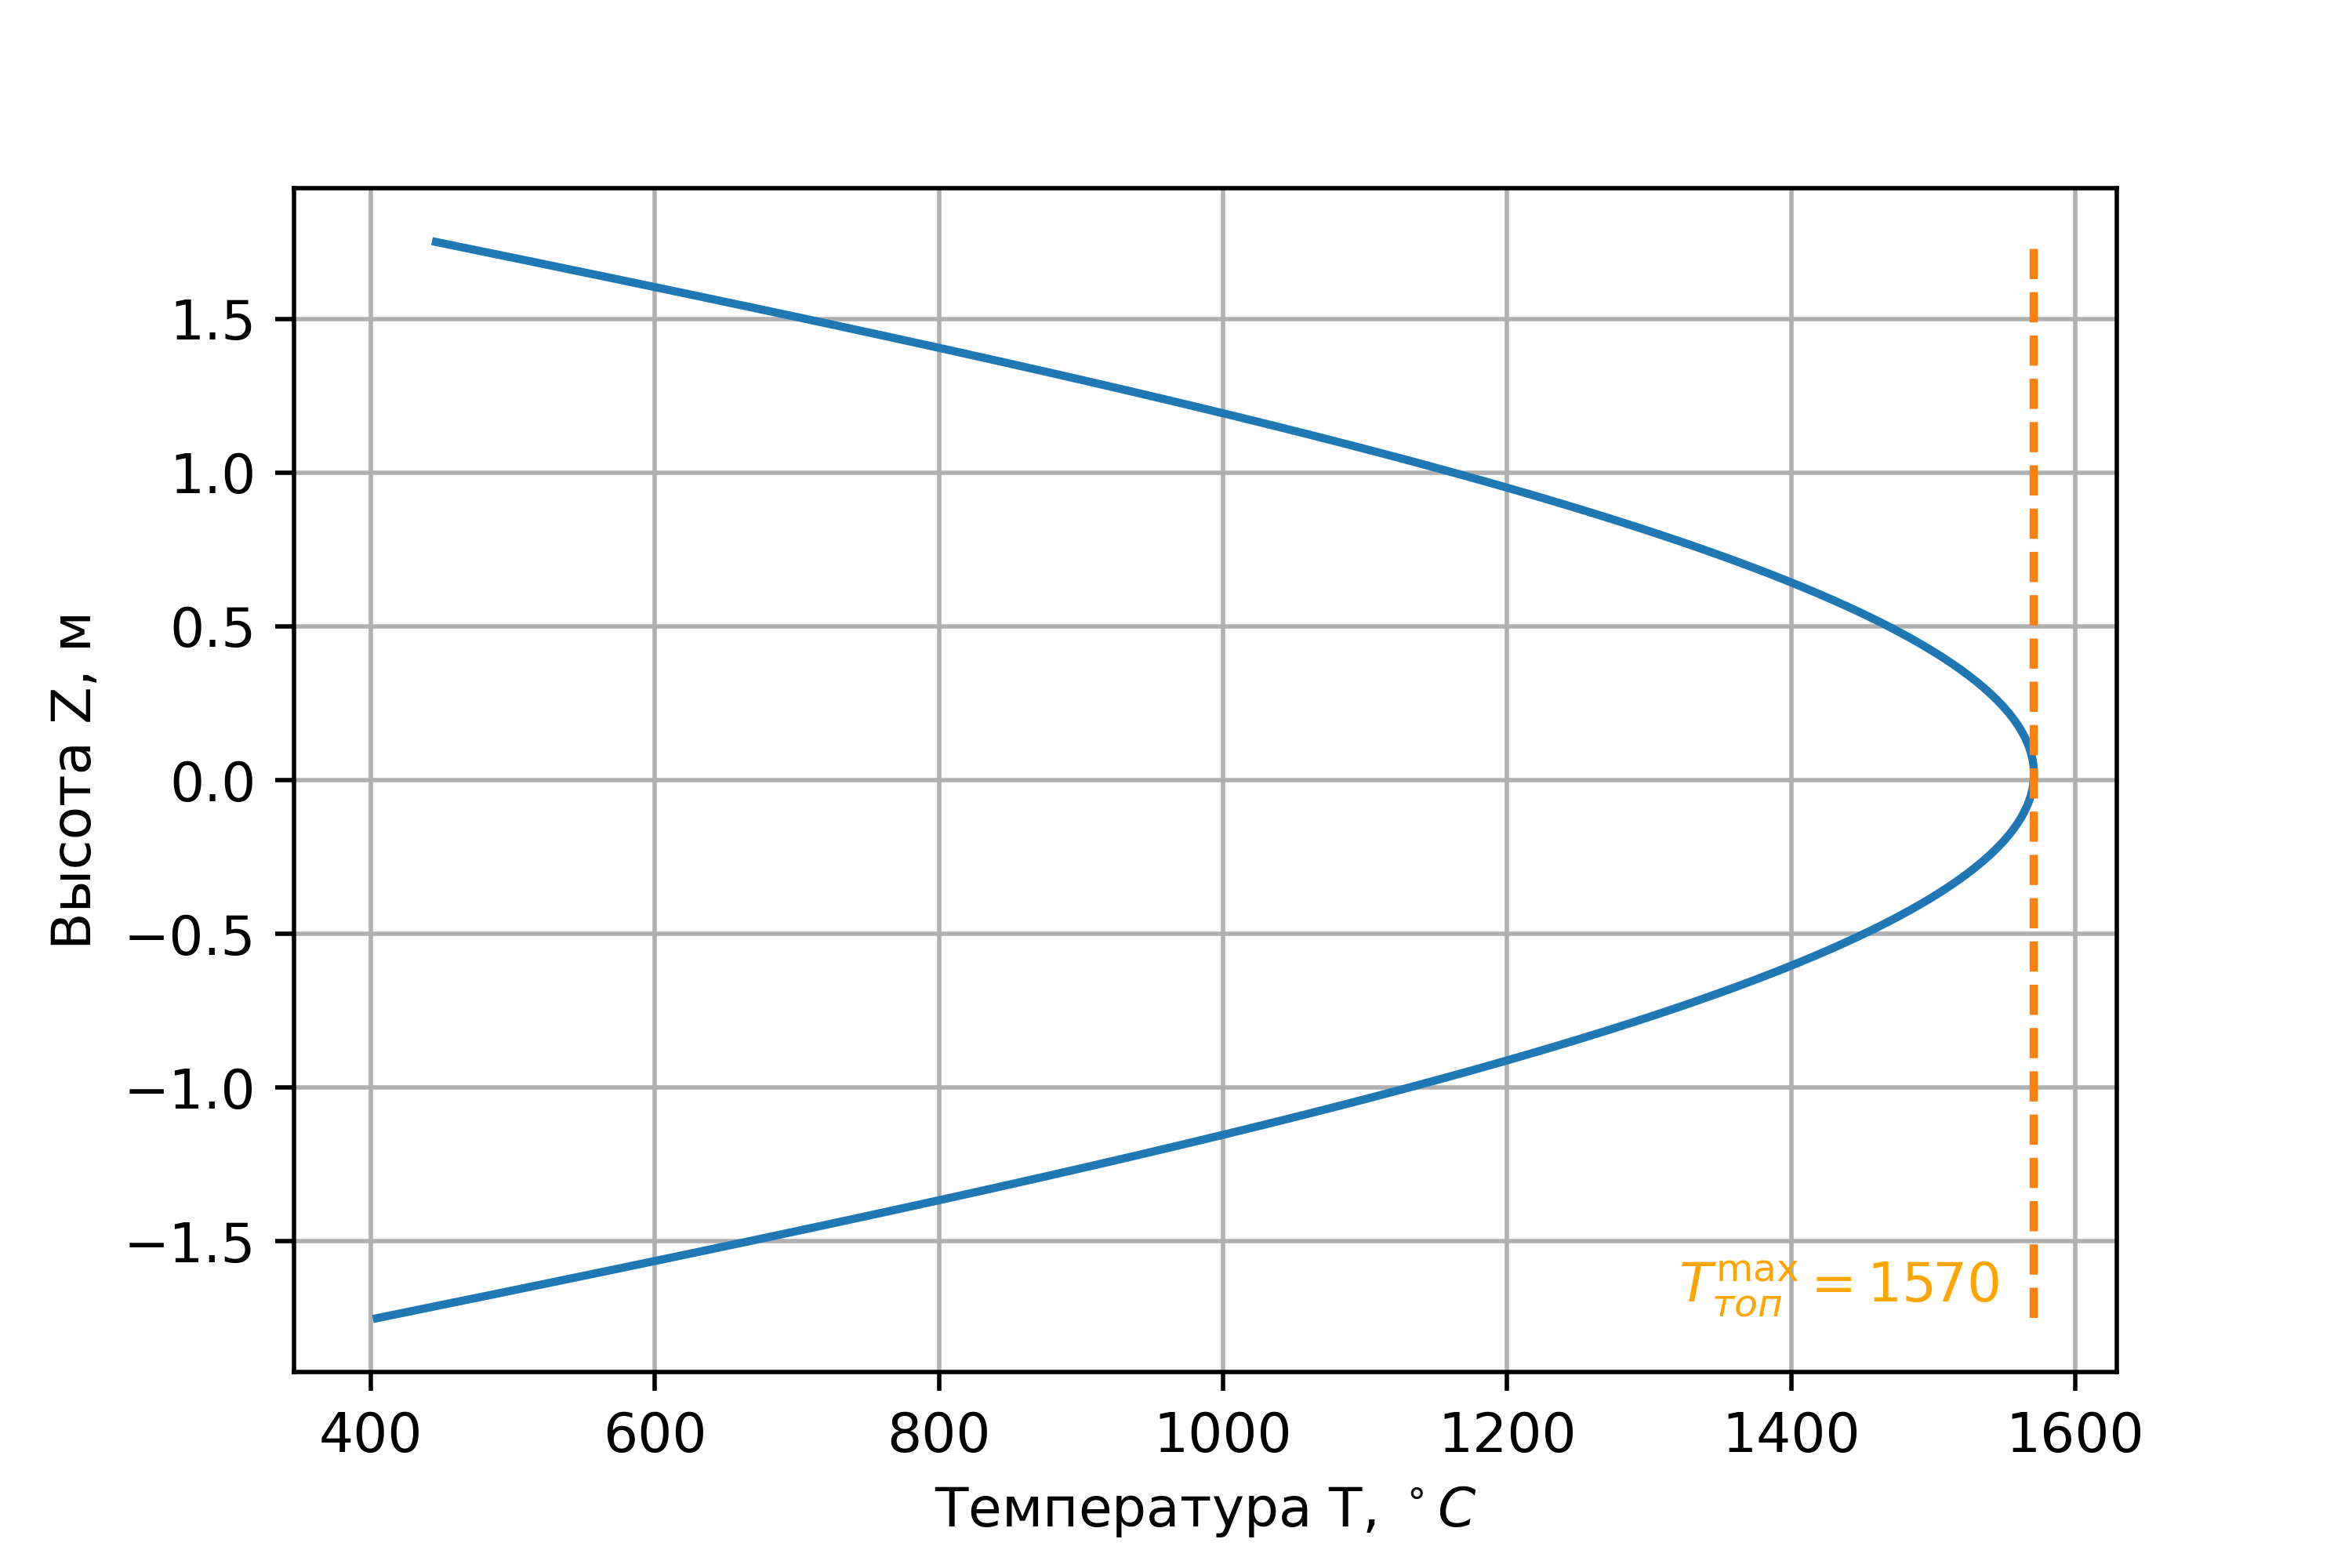
\includegraphics[]{Ttop.png}
		\caption{Изменение температуры топлива по высоте}
		\label{pic:top} % название для ссылок внутри кода
	\end{center}
\end{figure}

Максимальная температура топлива $T_{\text{топ}} = 1559 ^\circ C$ при $Z_{\text{max}} = 0 \text{м}$. Максимально допустимая температура топлива при авариях определяется температурой плавления оксида урана и составляет с некоторым запасом $2600 ^\circ C$. Однако в условиях нормальной эксплуатации максимально допустимая температура топлива определяется сколонностью топлива к усиленному распуханию. % начиная с некоторой температуры, которая равна $1041 ^\circ C$.

\subsection{Определение перепадов давления и необходимой мощности насосов на прокачку}
Для того чтобы определить мощность на прокачку теплоносителя через реактор, найде перепад давления в ТВС
\noindent Гидравлическое сопротивление трения по формуле Дарси:
$$
\Delta P_{\text{тр}}=\xi_{\text{тр}}\cdot\frac{H_{\text{аз}}}{d_{\text{г}}}\cdot \frac {w^2}{2}\rho_{\text{ср}}
=
1.349 \cdot 10^{ -02 } \frac {3.500 } {9.263 \cdot 10^{ -03 }} \cdot \frac {(5.629 )^2} {2} \cdot 7.165 \cdot 10^{ 2 }
=5.785 \cdot 10^{ 4 } \text{Па}
$$
где 
\begin{itemize}
\item $w$, средняя скорость теплоносителя: \begin{equation}w = \frac{G_{\text{реак}}}{\rho_{\text{ср}} \cdot S_{\text{прох}} \cdot N_{\text{ТВС}}}= \frac {1.579 \cdot 10^{ 4 }} {7.165 \cdot 10^{ 2 } \cdot 2.402 \cdot 10^{ -02 } \cdot 1.630 \cdot 10^{ 2 }} = 5.629 \ \text{м} /\text{c}\end{equation}
\item $\rho_{\text{ср}} = 720\ \text{Па}$ — средняя плотность среды
\end{itemize}

\noindent Потеря напора на ускорение:
\begin{equation}
\Delta P_{\mathrm{уск}} = \left( \frac{G_{\text{реак}}}{N_{\mathrm{TBC}} \cdot S_{\mathrm{npox}}} \right)^{2} \cdot \left(\frac{1}{\rho_{\mathrm{вых}}} - \frac{1}{\rho_{\mathrm{вx}}} \right)
=
\left( \frac{ 1.579 \cdot 10^{ 4 } } { 1.630 \cdot 10^{ 2 } \cdot 2.402 \cdot 10^{ -02 } } \right)^2 \cdot \left(\frac 1 { 6.808 \cdot 10^{ 2 } } - \frac 1  { 7.521 \cdot 10^{ 2 } } \right) =  2.265 \cdot 10^{ 3 } \text{Па}
\end{equation}, где $\rho_{\text{вых}} = 680.8\ \frac{\text{кг}}{\text{м}^2} $, $\rho_{\text{вх}} =752.1\  \frac {\text{кг}}{\text{м}^2}$.
\newline
\noindent Нивелирный напор:
$$
\Delta P_{\text{нив}} = \rho_{\text{ср}} \cdot g \cdot H_{\text{аз}}
=
7.165 \cdot 10^{ 2 } \cdot 9.807 \cdot 3.500  = 2.459 \cdot 10^{ 4 } \text{Па}
$$
Местное сопротивление:
$$
\Delta P_{\text{мест}} = \frac{ \left( \frac{1.579 \cdot 10^{ 4 }} {163 \cdot 2.402 \cdot 10^{ -02 } }  \right)^2 } {2} \cdot \left( \frac{ 2.6 }{ 7.521 \cdot 10^{ 2 } } +\frac{ 13 \cdot 0.45 }{7.165 \cdot 10^{ 2 }}+\frac{0.26} { 6.808 \cdot 10^{ 2 } } \right) = 9.761 \cdot 10^{ 4 } \text{Па}
$$
где $\xi_{\text{вх}}= 2.6 $ — коэффициент сопротивления на входе в кассету; $\xi_{\text{вых}} = 0.26$ — коэффициент сопротивления на выходе из кассеты, $\xi_{\text{реш}} = 0.45$ — коэффициент сопротивления при проходе через дистанцирующую решетку %укажи количество дистанцирующих решеток
Общее сопротивление каналов:
$$
\Delta P=\Delta P_{\mathrm{тр}}+\Delta P_{\mathrm{уск}}+\Delta P_{\text { нив }}+\Delta P_{\text {мест }} = 1.823 \cdot 10^{ 5 } \text{Па} 
$$
Мощность, необходимая для прокачки теплоносителя через весь реактор:
$$
N_{\mathrm{пр}}=N_{\mathrm{ТВС}} \frac{\Delta P \cdot G_{\mathrm{TBC}}}{\eta_{\text {нас }} \cdot \rho_{\mathrm{вх}}}
$$, где $\eta_{\text{нас}}=0.8$ — КПД насоса
\[
    N_{\text{пр}} = 163 \cdot \frac {1.823 \cdot 10^{ 5 } \cdot 9.685 \cdot 10^{ 1 }} {0.8 \cdot 7.521 \cdot 10^{ 2 }} = 4.783 \cdot 10^{ 6 } \text{Вт}
\]
\noindent КПД реактора с учетом потерь на прокачку теплоносителя:
$$
\eta^{\prime} = \frac{Q_{\text {эл }}-N_{\text {пр }}}{Q_{\text {теп }}}=\frac{1.000 \cdot 10^{ 9 } - 4.783 \cdot 10^{ 6 }}{2.904 \cdot 10^{ 9 }}={3.427 \cdot 10^{ -01 }}
$$
% \subsection{Определение запаса до кризиса теплообмена}
\subsection{Выводы из теплофизического расчета}
По итогам теплогидравлического расчета были определены основные термодинамические и теплогидравлические параметры РУ ВВЭР-1000. Были выполнены следующие поставленные задачи:
\begin{enumerate}
   \item Произведен выбор турбины и определён её КПД равный 0.342 с учетом мощности, необходимой на прокачку теплоносителя.
   \item Были найдены зависимости температуры оболочки и теплоносителя от высоты АЗ, было выяснено, что поверхностного кипения не наблюдается, и максимальная тепература оболочки твэла 341.6 $^\circ C$ не превышает предельно допустимую.
   \item Определена зависимость температуры топлива от высоты АЗ, максимальная температура топлива $1464 ^\circ C$ не превышает предельное значение $1900 ^\circ C$.
\end{enumerate}

% \section{Нейтронно-физический расчет}